\section{Analysis 1a}

    \subsection{Reelle Zahlen}
	
		\begin{tabular}{l l l}
			$\mathbb{N}$  & \{1, 2, 3, 4, ...\} & ganze Zahlen \\
			$\mathbb{N}_0$ & \{0, 1, 2, 3, ...\} = $\mathbb{N}$ $\cup$ \{0\} & ganze Zahlen inkl. 0 \\
			$\mathbb{Z}$ & \{$\pm1, \pm2, \pm3 $\} $\cup$ \{0\} & natürliche Zahlen \\
			$\mathbb{Q}$ & \{$ \frac{p}{q} | p \in \mathbb{Z} \wedge q \in \mathbb{Z} \setminus $\{0\}\} & rationale Zahlen \\
			$\mathbb{R}$ & & ergänzt $\mathbb{Q}$ durch irr. Zahlen \\
			             & & wie $\sqrt{2}$, reelle Zahlen \\
			$\mathbb{R} \setminus \mathbb{Q}$ & & Irrationale Zahlen \\
		\end{tabular}

		\subsubsection{Supremum und Infimum}
			\begin{tabular}{ll} 
				sup(X) & kleinste obere Schranke  \\
				       & Maximum ist immer auch Supremum \\
				\\
				inf(X) &  grösste untere Schranke \\ 
				       & Minimum ist immer auch Infimum \\
			\end{tabular}			
				
		\subsubsection{Binomischer Satz / Binomialkoeffizient}	
			\begin{tabular}{ll} 
				Pascal-Dreieck berechnen:  & $\left(a+b\right)^n = \sum\limits _{k=0}^n \binom{n}{k}a^{n-k}\cdot b^k$ \\
				$\binom{n}{k}=\binom{n}{n-k}$ & $\binom{n}{k-1}+\binom{n}{k}=\binom{n+1}{k}$ \\
				\\
				$\binom{n}{k}=\frac{n!}{k!\left(n-k\right)!}$ & $\binom{n}{k} = 0$ wenn k $<$ 0 oder k $>$ n \\ 
				\\
				$\binom{n}{0}=1$ &  $\binom{n}{n}=1$ \\ 	 		
			\end{tabular}				 
				 
		\subsubsection{Umgebung}
			\begin{tabular}{ll} 
				Jedes offene Intervall, dass die Zahl a enthält, & \\ 
				heisst eine Umgebung von a                       &  U(a)\\
				\\
				Es sei $\epsilon >$ 0. Unter der $\epsilon$-Umgebung von a & \\ 
				versteht man das offene Intervall $(a-\epsilon,a+\epsilon)$ &  $U_\epsilon(a)$\\ 
				\\
				Eine $\epsilon$-Umgebung von a ohne die Zahl a selbst & \\ 
				wird punktierte $\epsilon$-Umgebung von a genannt & $\dot{U}_\epsilon(a)=U_\epsilon(a)\smallsetminus{a}$ \\ 
			\end{tabular}
			
		\subsubsection{Spezielle endliche Reihen}
			\begin{tabular}{ll} 
				arithmetisch: & $\sum\limits _{i=1}^n i = \frac{n(n+1)}{2}$ \\
				\\
				geometrisch: & $\sum\limits _{i=0}^n q^i = \frac{q^{n+1} - 1}{q - 1}$ \\
			\end{tabular}
				
		\subsubsection{Mittelwerte}
			\begin{tabular}{ll} 
				Harmonisches Mittel (HM) : &  $\frac{1}{\frac{1}{n}(\frac{1}{a_1}+\frac{1}{a_2}+...+\frac{1}{a_n})}$ \\
				\\
				Geometrisches Mittel (GM) : & $\sqrt[n]{a_1 a_2 \ldots a_n}$ \\
				\\
				Arithmetisches Mittel (AM) : & $\frac{1}{n} \cdot \sum\limits _{i=1}^n a_i = 	\frac{a_1+a_2+...+a_n}{n}$ \\
			\end{tabular}
			
		\subsubsection{Spezielle Ungleichungen}
			\begin{tabular}{ll} 
				Bernoulli-Ungleichung: & $(1 + a)^n > 1 + n \cdot a$\\
				                       & für $n \in N, n \geq 2, a \in R, a > -1, a\neq0$ \\
				\\
				Binomische Ungleichung: & $|a\cdot b|\leq\frac{1}{2}(a^2 + b^2)$\\ 
				\\
				Mittelungleichung: & $ HM \leq GM \leq AM $\\
				\\
				Gleichheit: & $ HM = GM = AM$ \\
				            & für $a_1 = a_2 = ... = a_n$ \\
				\\
				Dreiecksungleichungen: & $\left|a+b\right|\leq\left|a\right|+\left|b\right|$ \\
				                       & 	$\left|a-b\right|\leq\left|a\right|+\left|b\right|$  \\
				                       & $\left|a-b\right|\geq\left|\left|a\right|-\left|b\right|\right|$ \\
			\end{tabular}
				
		\subsubsection{Vollständige Induktion}	
			\begin{tabular}{lll} 
				Verankerung VA: & Beweise Formel für $a_0$ & \\
				Vererbung VE:   & (1) Annahme: & Formel gilt für $a_n$ \\
				                & $\downarrow$ & \\
				                & (2) Schritt: & Formel gilt auch für $a_{n+1}$ \\
			\end{tabular}
				
			Mittels Berechnung soll bewiesen werden, dass (2) ebenso gilt wie (1) \\

			\textbf{Beispiel:} \\
			
			\begin{tabular}{llll} 
				(VA) & $\sum \limits_{i=1}^1 i = \frac{1(1+1)}{2} = 1 $ \\
				(VE) (1) & $\sum \limits_{i=1}^n i = \frac{n(n+1)}{2}$  \\
				(VE) (2) & $\sum \limits_{i=1}^{n+1} i = \frac{(n+1)(n+1 + 1)}{2} = \frac{(n+1)(n+2)}{2} $  \\
			\end{tabular}
	
	\subsection{Funktionen}

		Schreibweisen: \\
		$f:D_f \rightarrow W_f$ mit $x \mapsto f(x)$\\
		$f:x \mapsto f(x)$ mit $x \in D_f$\\
		$y=f(x)$ mit $x \in D_f$		 \\	
		\\
		\begin{tabular}{ll}
			Monoton wachsend:   & $x_1 < x_2 \Rightarrow f(x_1) \leqq f(x_2)$ \\
			Monoton sinkend:    & $x_1 > x_2 \Rightarrow f(x_1) \geqq f(x_2)$ \\
			Monoton streng ...: & Siehe oben, jedoch immer $f(x_1) < f(x_2)$ bzw. $f(x_1) > f(x_2)$ \\
			Beschränktheit:     & Funktion besitzt obere oder untere Grenze, meist inf oder sup \\
			Umkehrbarkeit:      & Streng monotone Funktionen sind umkehrbar, pro $x$ ein $y$ und umgekehrt \\
			Restriktion:        & Nur einen Teil von $D_f$ betrachten \\ 
				                & $\Rightarrow$ Umkehrbarkeit \\
		\end{tabular}
						
		\subsubsection{Transformationen}	
			\begin{tabular}{lll}
				1. & Streckung um \textbf{1/a} in x-Richtung & $y = f(a \cdot x)$ \\
				   & Spiegelung an y-Achse bei \textbf{-a} & \\
				2. & Verschiebung nach links (\textbf{+b}) oder rechts  (\textbf{-b}) & $y = f(x \pm b)$\\
				3. & Streckung um \textbf{c} in y-Richtung & $y = c \cdot f(x)$ \\
				   & Spiegelung an x-Achse bei \textbf{-c} & \\
				4. & Verschiebung nach oben (\textbf{+d}) oder unten (\textbf{-d}) & $y = f(x) \pm d $ \\
			\end{tabular}
			
		\subsubsection{Spezielle Funktionen}
			\textbf{Identität:} \\
				\begin{tabular}{lll}
					$f(x) = x$ & &  y-Wert ist gleich dem x-Wert 
				\end{tabular}
			\\
			\textbf{Signum-Funktion:} \\
				Vorzeichenfunktion $f(x)=sgn(x)$\\
				$y= \left\{\begin{array}{l}\text{1, falls $x>0$} \\
					                       \text{0, falls $x=0$} \\
					                       \text{-1, falls $x<0$}\end{array}\right.$
			\\	
			\textbf{Floor-Funktion:} \\
			 	Abrunden auf nächste ganze Zahl \\
			
				\begin{tabular}{lll}
					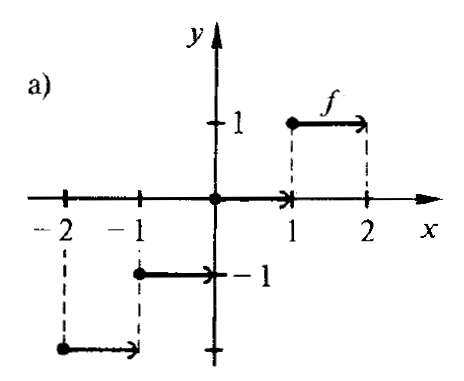
\includegraphics[height=3cm]{Bilder/floor-funktion} & &  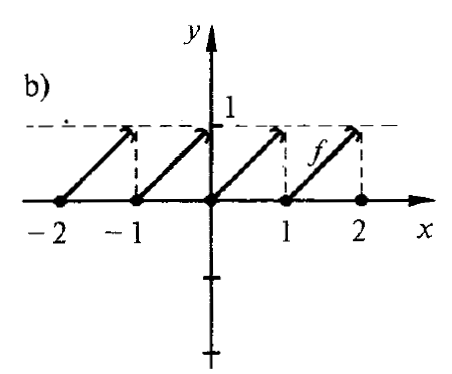
\includegraphics[height=3cm]{Bilder/saegezahn-funktion} \\
					Schreibweise: \textbf{$[x]$}                        & &  Schreibweise: \textbf{$x - [x]$} \\
				\end{tabular}
			
		\subsubsection{Schwingungen}
			Sinus-Schwingung:  $y = A \cdot \sin(\omega \, t + \phi)$ \\
			
			\begin{tabular}{llllllll}
				$A$ & Amplitude & & $\omega$ & Frequenz $\frac{2 \pi}{\mathrm{sec}}$ & & $\varphi$ & Phase \\
			\end{tabular}			
			
			\textbf{Superposition von Schwingungen} \\
			$y = A \cdot \sin(\omega \, t + \varphi)  =  A_1 + A_2 \cdot \sin(\omega \, t + \varphi_1 + \varphi_2)$\\ 
			\\
			$A = \sqrt{A_1^2 + A_2^2 + 2 \,A_1 \cdot A_2 \cdot \cos(\varphi_1 - \varphi_2)}$
			
		\subsubsection{Verkettung oder mittelbare Funktion}
			\begin{tabular}{ll} % Tabelle mit 2 Sptalten
				g nach f: & \\
				$h(x)=g \circ f \Rightarrow h(x)=g(f(x))$ & $W_h=W_g \rightarrow D_h=D_f$ \\
				\\
				f nach g: \\
				$h(x)=f \circ g \Rightarrow h(x)=f(g(x))$ & $W_h=W_f \rightarrow D_h=D_g$ \\				
			\end{tabular}
			
		\subsubsection{Gerade / ungerade Funktionen}
			\begin{tabular}{lll} 
				 gerade:     & $f(-x) = f(x)$      & symmetrisch zu y-Achse \\
				 ungerade:   & $f(-x) = -f(x)$     & punktsymmetrisch \\
				 periodisch: & $f(x) = f(x \pm p)$ & wiederholend mit Periode p \\								
			\end{tabular}			
				
		\subsubsection{Ganzrationale Funtkionen (Polynome)}
			Aussehen: $f(x)=a_nx^{n}+a_{n-1}x^{n-1}+\cdots+a_1x+a_0$\\
			\\
			\textbf{Nullstellen bestimmen:} \\
			Quadratische Funktion: $x_1 , x_2 = \frac{-b \pm \sqrt{b^2 - 4ac}}{2a}$ \\
			\\
			Faktorisierung mit Binomen / Hornerschema \\
			\\
			Eine Funktion vom Grad n hat höchstens n verschiedene Nullstellen!
			
		\subsubsection{Gebrochenrationale Funktionen}
			Aussehen: $f(x)=\frac{p_m(x)}{q_n(x)}=\frac{a_mx^{m}+a_{m-1}x^{m-1}+\cdots+a_1x+a_0}{a_nx^{n}+a_{n-1}x^{n-1}+\cdots+a_1x+a_0}$ \\
			
			\begin{tabular}{ll} 
				m & Zählergrad \\
				n & Nennergrad \\
				$m < n$ & echt gebrochen \\
				$m = n$ & gleichgradig \\
				$m > n$ & unecht gebrochen \\ 
			\end{tabular}	
		
			Jede unecht gebrochene Funktion lässt sich als Summe einer ganzrationalen Funktion und einer echt gebrochenen Funktion schreiben. \\
			$\Rightarrow$ Polynomdivision \\

		\subsubsection{Hornerschema}
			Zerlegt eine ganzrationale Funktion vom Grad n in einen Linearfaktor (Nullstelle) und ein Polynom vom Grad n-1 \\
			
			\begin{tabular}{ll}
				1. & Nullstelle $x_0$ raten \\
				2. & Von oben nach unten summieren \\
				3. & Diagonal nach rechts mit $x_0$ multiplizieren \\
			\end{tabular}	
			
			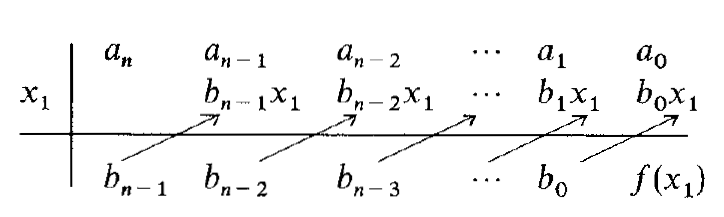
\includegraphics[width=0.7\linewidth]{Bilder/hornerschema_allg}
					
			\textbf{Beispiel:}
			
			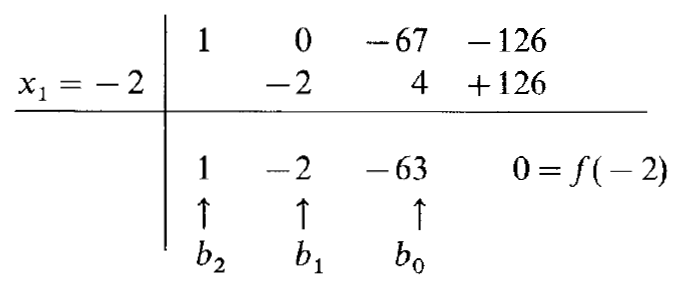
\includegraphics[height=2cm]{Bilder/hornerschema_bsp}

				$f(x) = x^3-67x-126$\\
				$\Rightarrow f(x) = (x-x_1)(b_2x^2 + b_1x + b_0) = (x+2)(x^2-2x-63)$ 
			
		\subsubsection{Polynomdivision}
			Liefert Summe aus ganzrationaler Funktion und echt gebrochener Funktion\\
			\\
			\textbf{Beispiel:}\\
				\vspace{-5pt} \polylongdiv[style=C]{-2x^2-x-1}{x-1} \\
			
		\subsubsection{Partialbruchzerlegung}
			\begin{tabular}{ll}
				(1) & echt gebrochen (Zähler < Nenner) \\
				    & Ja: $\rightarrow$ (2) \\
					& Nein: $\rightarrow$ Polynomdivision \\
				(2) & Nenner faktorisieren \\
				    & pro Faktor ein Teilbruch \\
				(3) & Berechnung Zählerkonstanten \\
				(3.1) & Gleichnamig machen (kgV) \\
				(3.2) & Zählergleichung \\
				(3.3) & Einsetzen von "guten"  x-Werten \\			
			\end{tabular}
			
			\textbf{Beispiel PBZ} \\
				\begin{tabular}{ll}
					(1) & $f(x) = \frac{1}{a^2 - x^2}$ \\
					\\
					(2) & $a^2 - x^2 = (a+x)(a-x)$ \\
					\\
					(3) & $\frac{A}{a+x} + \frac{B}{a-x} = \frac{1}{a^2 - x^2}$\\
					\\
					(3.1) & $\frac{A(a-x) + B(a+x)}{a^2 - x^2} = \frac{1}{a^2 - x^2}$ \\
					\\
					(3.2) &$ A(a-x) + B(a+x) = 1$ \\
					\\
					(3.3) & $x = a \Rightarrow B(2a) = 1 \Rightarrow B = \frac{1}{2a} $ \\			
					& $x = -a \Rightarrow A(2a) = 1 \Rightarrow A = \frac{1}{2a} $ \\
				\end{tabular}
			\\
			\textbf{Spezielle Ansätze PBZ} \\
				\begin{tabular}{ll}
					$f(x)$ & $=\frac{5x^2-37x+54}{x^3-6x^2+9x} =  \frac{A}{x}+\frac{B}{x-3}+\frac{C}{(x-3)^2}$ \\ 
					       & $=\frac{A(x-3)^2+Bx(x-3)+Cx}{x(x-3)^2}$ \\
					\\
					$f(x)$ & $=\frac{1,5x}{x^3-6x^2+12x-8}=\frac{A}{x-2}+\frac{B}{(x-2)^2}+\frac{C}{(x-2)^3}$ \\
					       & $=\frac{A(x-2)^2+B(x-2)+C}{(x-2)^3}$ \\
					\\
					$f(x)$ & $=\frac{x^2-1}{x^3+2x^2-2x-12}=\frac{A}{x-2}+\frac{Bx+C}{x^2+4x+6}$ \\
					       & $=\frac{A(x^2+4x+6)+(Bx+C)(x-2)}{(x-2)(x^2+4x+6)}$ \\
				\end{tabular}
		
		\subsubsection{Trigonometrie, Arcus}
			\begin{tabular}{llll}
				$\sin(x)$: & $D_f=[-\frac{\pi}{2},\frac{\pi}{2}]$ & $\rightarrow$ &  $W_f=[-1,1]$ \\
				$\cos(x)$: & $D_f=[0,\pi]$ & $\rightarrow$ &  $W_f=[-1,1]$  \\
				$\tan(x)$: & $D_f=(-\frac{\pi}{2},\frac{\pi}{2})$ & $\rightarrow$ & $W_f=\mathbb{R}$\\
				$\cot(x)$: & $D_f=(0,\pi)$ & $\rightarrow$ &  $W_f=\mathbb{R}$ \\
				\\
				$\arcsin(x)$: & $D_f=[-1,1] $ & $\rightarrow$ & $ W_f=[-\frac{\pi}{2},\frac{\pi}{2}]$ \\
				$\arccos(x)$: & $D_f=[-1,1]$ & $\rightarrow$ &  $W_f=[0,\pi]$ \\
				$\arctan(x)$: & $D_f=\mathbb{R}$ & $\rightarrow$ &  $W_f=(-\frac{\pi}{2},\frac{\pi}{2})$ \\
				$\mathrm{arccot}(x)$: & $D_f=[-1,1]$ & $\rightarrow$ &  $W_f=(0,\pi)$ \\		
			\end{tabular}

			\paragraph{Umwandlung}
				\begin{tabular}{ll}
					$\sin(x + \frac{\pi}{2}) = \cos(x)$ & $\cos(x - \frac{\pi}{2}) = \sin(x)$ \\	
				\end{tabular}

			\paragraph{Pythagoras}
				\begin{tabular}{ll}
					$\sin^2(x) + \cos^2(x) =$ & $ 1 $ \\
				\end{tabular}

			\paragraph{2 Winkel}
				\begin{tabular}{ll}
					$\cos(\alpha \pm \beta)$ & $= \cos\alpha\cos\beta \mp \sin\alpha\sin\beta$ \\
					$\sin(\alpha \pm \beta)$ & $= \sin\alpha\cos\beta \pm \sin\beta\cos\alpha$ \\
				\end{tabular}

			\paragraph{Summenformel}
				\begin{tabular}{ll}
					$\sin\alpha + \sin\beta$ & $= 2 \cdot \cos(\frac{\alpha - \beta}{2}) \cdot \sin(\frac{\alpha + \beta}{2})$ \\
				\end{tabular}
			
			\paragraph{Symmetrien} 
				\begin{tabular}{ll}
					Sinus & Punkt $(0|0) \rightarrow \sin(-x) = - \sin(x)$ \\
					      & Scheitelsymm. $\rightarrow \sin(\frac{\pi}{2} + x) = \sin(\frac{\pi}{2} - x)$ \\
					      & Punkt $\rightarrow \sin(\pi - x) = \sin(x)$ \\
					\\
					Cosinus & y-Achse $\rightarrow \cos(-x) = \cos(x)$ \\
					        & Scheitel $\rightarrow \cos(\pi - x) = \cos(\pi + x)$ \\		
				\end{tabular}
				
		\subsubsection{Winkel zwischen beliebigen Geraden}
			\begin{tabular}{ll}
				Zwischenwinkel: & $\tan(\alpha) = \frac{m_1 - m_2}{1 + m_1 \cdot m_2} \rightarrow$ Winkel geg. Uhrzeiger \\
				                & 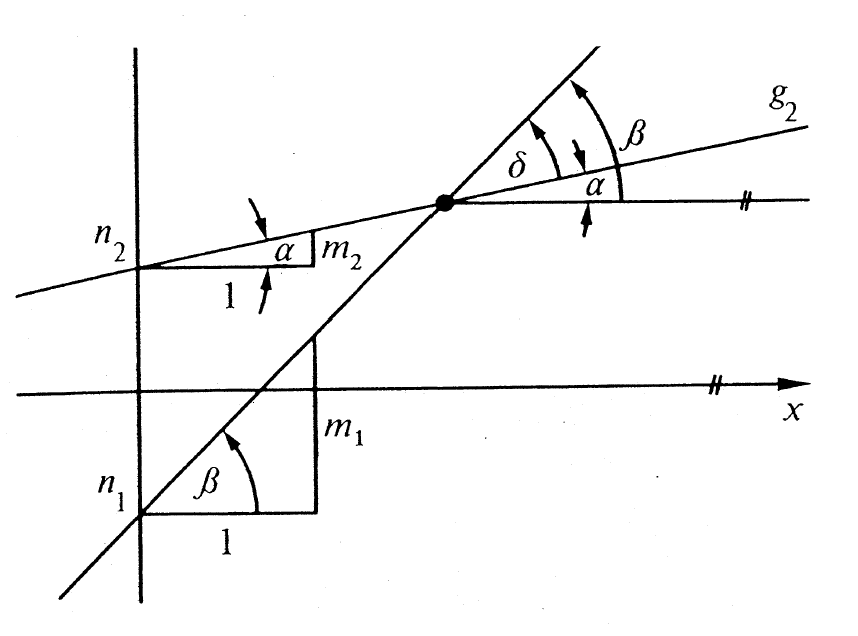
\includegraphics[width=0.3\linewidth]{Bilder/zwischenwinkel.png}\\
				Senkr. Geraden: & $m_1 \cdot m_2 = -1$ \\
			\end{tabular}
            
	\subsection{Folgen und Reihen}
			
		\subsubsection{Spezielle Folgen und Reihen}
			\begin{tabular}{lll}
				Arithmetische Folge: & $a_{n+1} = a_n + d$ & $d = a_{n+1} - a_n$ \\
				\\
				Geometrische Folge: & $a_{n+1} = q \cdot a_n $ & $q = \frac{a_{n+1}}{a_n}$ \\
				\\
				Konstante Folge: & $a_{n+1} = a_n$  & \\
			\end{tabular}				
				
		\subsubsection{Beschränktheit / Monotonie}
			\paragraph{Beschränktheit}
				$W_f \subset [a ; b]$ und a, b $\in \mathbb{R}$		
			
			\textbf{Monotonie:} \\
			
			\begin{tabular}{|c|c|c|c|}
				\hline
				$f(x_1) \leq f(x_2)$ & $x_1 < x_2$ & monoton wachsend & $\uparrow$\\
				\hline
				$f(x_1) < f(x_2)$ & $x_1 < x_2$ & streng monoton wachsend & $\Uparrow$\\
				\hline
				$f(x_1) \geq f(x_2)$ & $x_1 > x_2$ & monoton fallend & $\downarrow$\\
				\hline
				$f(x_1) > f(x_2)$ & $x_1 > x_2$ & streng monoton fallend & $\Downarrow$\\
				\hline
			\end{tabular}
			
		\subsubsection{Konvergenz, Divergenz}
			\textbf{Konvergenz} \\
				Es existiert ein Grenzwert g $\in \mathbb{R}$ \\
				Toleranzungleichung: $\vert a_n - g \vert < \epsilon$  mit $\epsilon > 0$ \\
				Gesucht ist ein $n_0$, ab welchem alle Werte von $n \geq n_0$ in $U_\epsilon(g)$ liegen \\
				
			\textbf{Bestimmt divergent gegen +$\infty$} \\
				Ungleichung: $f_n > K$ wenn $n \geq  n_0$ f"ur $K > 0$ 
				
			\textbf{Bestimmt divergent gegen -$\infty$} \\
				Ungleichung: $f_n < k$ wenn $n \geq  n_0$ f"ur $k < 0$ 
				
			\textbf{Unbestimmt divergent} \\
				Alles, was nicht konvergent oder bestimmt divergent ist
				
		\subsubsection{Grenzwerte gegen Unendlich}
			Vorgehen beim lösen von Grenzwerten \\
				\begin{tabular}{ll}
					1. & Naiven Ansatz ausprobieren $\rightarrow$ limit direkt bilden \\
					2. & Falls unbestimmte Form entsteht: \\
					   & Umformen gemäss folgenden Ansätzen \\
				\end{tabular}
				
				\begin{tabular}{ll}
					Arithmetik:  & $+, -, *, :, \sqrt{...}, \vert ...\vert$ \\
					Erweiterung: & erweitern mit $\frac{1}{x^n}$ n = h"ochste (Nenner-)Potenz \\
					Erweiterung: & erweitern mit Gegentherm (3. Binom bilden)\\
					Tabelle:     & Bei Br"uchen Tabelle aus Abschnitt 4.8 anschauen! \\
				\end{tabular}

			\textbf{Beispiel Grenzwert n gegen Unendlich} \\
				$f(n) = \frac{-2n^2+4n-5}{8n^2-3n+7}$ $(n \rightarrow \infty)$ \\
				\\
				"Naiv": $\frac{-\infty + \infty + 5}{\infty - \infty + 7} \rightarrow \frac{-\infty + \infty}{\infty - \infty} \rightarrow \frac{?}{?}$ \\
				\\
				Algebra, Erweitern mit $\frac{1}{n^2}$: $f(n) = \frac{-2+\frac{4}{n}-\frac{5}{n^2}}{8-\frac{3}{n}+\frac{7}{n^2}} (n \rightarrow \infty) = \frac{-2}{8} = -\frac{1}{4}$ \\				
		
		\subsubsection{Rechnen mit Unendlich}
			\textbf{Bestimmte Formen} \\
				\begin{tabular}{lll}
					$\infty + \infty = \infty$     & $-\infty - \infty = -\infty$          & $0 \cdot [a,b] = 0 \cdot \text{beschränkt} = 0$ \\
					\\
					$g + \infty = \infty$          & $g - \infty = -\infty$                & (g $\in \mathbb{R})$ \\
					\\ 
					$\infty \cdot \infty = \infty$ & $-\infty \cdot (\infty) = -\infty$    & $g \cdot \infty = 
						\begin{cases} 
							\infty & g > 0 \\ 
							-\infty & g < 0 
						\end{cases}$\\ 		
					\\
					$\frac{1}{\infty} = 0$         & $\frac{g}{\infty} = 0$                & $g \in \mathbb{R}$	\\
					\\
					$\frac{\infty}{0+} = \infty$   & $\frac{\infty}{0-} = -\infty$	       & $\frac{\infty}{g} = 
						\begin{cases}			
							\infty & g > 0 \\
							-\infty & g < 0
						\end{cases} $ \\
					\\
					$\frac{1}{0+} = \infty$        & $\frac{1}{0-} = -\infty$              & $g \in \mathbb{R} - {0}$ \\
				\end{tabular}

				\begin{tabular}{ll}
				$\frac{g}{0+} = \begin{cases}					
								\infty & g > 0 \\
								-\infty & g < 0
								\end{cases} $ &
				$\frac{g}{0-} = \begin{cases}				
								-\infty & g > 0 \\
								\infty & g < 0
								\end{cases}$ \\ 
				\end{tabular}
			
			\textbf{Unbestimmte Formen} \\
				\begin{tabular}{lll}
					$\frac{0}{0} = ?$    & $\frac{\infty}{\infty} = ?$ & $\infty \cdot 0 = ?$ \\
					\\
					$0 \cdot \infty = ?$ & $\infty - \infty = ?$       & $0^0 = ?$ \\
					\\
					$\infty^0 = ?$       & $1^{\infty} = ?$            & \\
				\end{tabular}
			
				Ausser 1 ist eine Konstante, dann gilt $1^{\infty} = 1 $ \\
				
		\subsubsection{Wachstumsvergleich} 
			\begin{tabular}{lll}
				(1) & $\frac{n^k}{q^n} (n \rightarrow \infty)= 0$  (k $\in \mathbb{N}; q > 1)$ & $\frac{\text{Potenz}}{\text{Exponentiell}} \rightarrow 0$\\
				\\
				(2) & $\frac{q^n}{n!} (n \rightarrow \infty)= 0$  (k $\in \mathbb{N}; q > 1)$  & $\frac{\text{Exponentiell}}{\text{Fakult"at}} \rightarrow 0$ \\
				\\
				(2) & $\frac{ln(n)}{n^k} (n \rightarrow \infty)= 0$  (k $\in \mathbb{N})$      & $\frac{\text{Logarithmisch}}{\text{Potenz}} \rightarrow 0$ \\
			\end{tabular}						
				
		\subsubsection{Bolzano-Prinzip}
			\textbf{Jede beschränkte, monotone Zahlenfolge ist konvergent!} \\
				\begin{tabular}{ll}
					1. & Monotonie beweisen \\
					2. &  Beschränktheit vermuten und möglichen Grenzwert g \\ 
					   & mittels Grenzwertgleichung finden  \\
					3. & Beschränktheit beweisen \\
					3.1 & $a_1$ ist obere/untere Schranke \\
					3.2 & Vermutete untere/obere Schranke mit voll. Induktion beweisen \\
					    & z.B. $a_{n+1} \leq a_n$ wobei $a_{n+1}$ und $a_n$ mit vermutetem \\
					    & Grenzwert ersetzt werden \\
				\end{tabular}
			
		\subsubsection{Exponentialfunktion}
			$\e = \lim\limits_{n \to \infty} (1+\frac{1}{n})^n $ \\
				\\
			\begin{minipage}{.45\linewidth}
				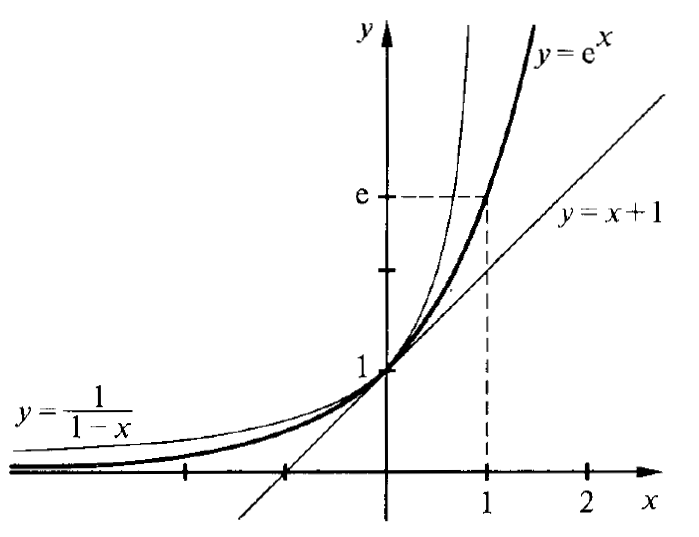
\includegraphics[width=0.95\linewidth]{Bilder/exp-funktion}
			\end{minipage}
			\hfill
			\begin{minipage}{.5\linewidth}
				Definitions- / Wertebereich: \\
				$D_f = \mathbb{R} \rightarrow W_f = \mathbb{R^+}$ \\
				\\
				Einschliessung: \\
					\begin{tabular}{ll}
					$\e^x \geq 1 + x$ & f"ur x $\in \mathbb{R}$ \\
					\\
					$\e^x \leq \frac{1}{1-x}$ & f"ur $x < 1$  \\
					\end{tabular}
			\end{minipage}

		\subsubsection{log-Rechenregeln}
			\begin{tabular}{|ll|ll|}
				\hline
				$ln(a \cdot b)$ & $= ln(a) + ln(b)$         & $ln(\frac{a}{b})$ & $= ln(a) - ln(b)$ \\
				\hline
				$e^{ln(a \cdot b)}$ & $= e^{ln(a) + ln(b)}$ & $ln(x^r)$         & $= r \cdot ln(x)$ \\
				\hline
				$a \cdot b$ & $= e^{ln(a)} \cdot e^{ln(b)}$ &                   &                   \\
				\hline
			\end{tabular}

		\subsubsection{Hyperbolische Funktionen}
			$\e^x = \frac{1}{2} (\e^x - \e^{-x}) + \frac{1}{2} (\e^x + \e^{-x}) = \sinh(x) + \cosh(x)$ \\
			\\
			\begin{tabular}{ll}
				$\sinh(x) = \frac{1}{2} (\e^x - \e^{-x})$ & $\mathbb{R} \rightarrow \mathbb{R}$ \\
				$\cosh(x) = \frac{1}{2} (\e^x + \e^{-x})$ & $\mathbb{R} \rightarrow [1; \infty)$ \\
				$\tanh(x)$ = $\frac{\sinh(x)}{\cosh(x)} = \frac{\frac{1}{2} (\e^x - \e^{-x})}{\frac{1}{2} (\e^x + \e^{-x})}$ & $\mathbb{R} \rightarrow (-1; 1)$ \\	
				$\vert \sinh(x) \vert < \cosh(x)$	& \\
			\end{tabular}
			
			\textbf{Area-Funktionen (Umkehrung Hyperbolische. F.)} \\
				\begin{tabular}{lll}
					$\mathrm{arsinh}(x): $ & $ln(x + \sqrt{x^2+1})$         & $\mathbb{R} \rightarrow \mathbb{R}$ \\
					$\mathrm{arcosh}(x): $ & $ln(x + \sqrt{x^2-1})$         & $[1; \infty) \rightarrow \mathbb{R}^+_0$  \\
					$\mathrm{artanh}(x): $ & $\frac{1}{2}ln\frac{1+x}{1-x}$ & $ \vert x \vert < 1 \rightarrow \mathbb{R} $ \\			
				\end{tabular}
			
		\subsubsection{Logarithmusfunktion}
				
			\begin{minipage}{.45\linewidth}
				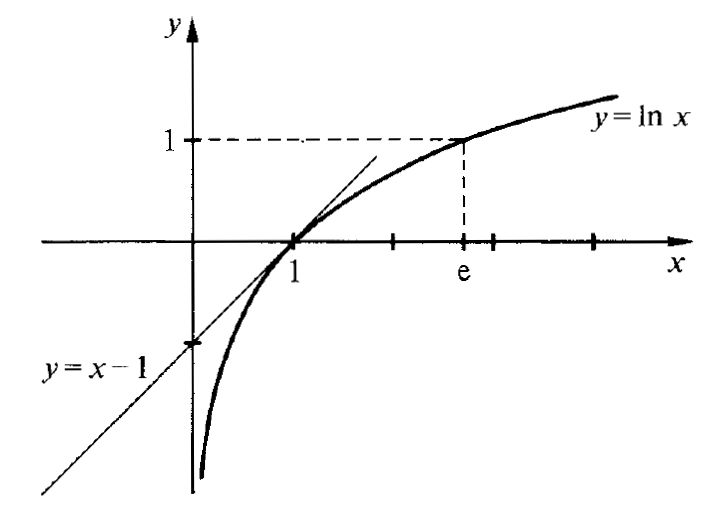
\includegraphics[width=0.95\linewidth]{Bilder/ln-funktion}
			\end{minipage}
				\hfill
			\begin{minipage}{.5\linewidth}
				Definitions- / Wertebereich: \\
				$D_f = \mathbb{R^+} \rightarrow W_f = \mathbb{R}$ \\
				\\
				Einschliessung: \\
				\\
				$1-\frac{1}{x} \leq \ln(x) \leq x-1$
			\end{minipage}
				
	\subsection{Grenzwerte von Funktionen}
			
		\subsubsection{Techniken zur Berechnung von Grenzwerten}	
			\begin{tabular}{ll}
				Arithmetik: & $+, -, *, :, \sqrt{...}, \vert ...\vert$ \\
				Erweiterung:& erweitern mit $\frac{1}{x^n}$ n = h"ochste (Nenner-)Potenz \\
				Erweiterung: & erweitern mit Gegentherm (3. Binom bilden)\\
				Faktorisierung: & Z"ahler und Nenner faktorisieren und kürzen \\
				%hier war mal Trigo: Bronstein S. 57 1.C, wurde jedoch nicht gefunden
			\end{tabular}
			
		\subsubsection{Links- / Rechtsseitiger Grenzwert}
			Eine kritische Stelle $x_0$ 	kann von links und rechts angen"ahert werden. \\
				
			\begin{tabular}{ll}
				linksseitiger Grenzwert: & $\lim\limits_{x \to x_0^-} f(x) = g^-$ \\
				\\
				rechtsseitiger Grenzwert: & $\lim\limits_{x \to x_0^+} f(x) = g^+$ \\
			\end{tabular}
			\\ 
			$\Rightarrow$ Wenn $g^- = g^+ = g \rightarrow$ Konvergenz  \\
			$\Rightarrow$ Wenn $g^- \neq g^+ \rightarrow$ unbestimmte Divergenz \\

		\subsubsection{Konvergenz, Divergenz}	
			\textbf{Konvergenz von f(x)} \\
		
				\begin{tabular}{lll}
					$x \rightarrow \infty$  & Toleranzungleichung: $\vert f(x) - g \vert < \epsilon$ & wenn $x > M(\epsilon)$ \\
					$x \rightarrow -\infty$ & Toleranzungleichung: $\vert f(x) - g \vert < \epsilon$ & wenn $x < m(\epsilon)$ \\
					\\
					$x \rightarrow x_0$     & Toleranzungleichung:  $\vert f(x) - g \vert < \epsilon$ & $ x \in \dot{U}_\delta(x_0)$ \\
				\end{tabular}
			
			\textbf{Bestimmte Divergenz von y = f(x)} \\

				\begin{tabular}{lll}
					\underline{Quadrant} & \underline{Kriterium} & \underline{Folgerung}  \\
					\Romannum{1}	 & 	$y \rightarrow \infty$ $(x \rightarrow \infty$) & $y > K$ wenn $x > M(K)$ \\
					\Romannum{2}	 & 	$y \rightarrow \infty$ $(x \rightarrow -\infty$) & $y > K$ wenn $x < m(K)$ \\
					\Romannum{3}	 & 	$y \rightarrow -\infty$ $(x \rightarrow -\infty$) & $y < k$ wenn $x < m(k)$ \\
					\Romannum{4}	 & 	$y \rightarrow -\infty$ $(x \rightarrow \infty$) & $y < k$ wenn $x > M(k)$ \\
					\\
					                 & 	$f(x) \rightarrow \infty$ & $y > K > 0$ wenn $ x \in \dot{U}_\delta(x_0)$ \\
					                 & 	$f(x) \rightarrow -\infty$ & $y < k < 0$ wenn $ x \in \dot{U}_\delta(x_0)$ \\
				\end{tabular}
		
		\subsubsection{Stetigkeit}
			Definition Stetigkeit: $\lim \limits_{x \to x_0} f(x) = f(x_0)$ \\
			Eine Funktion ist stetig, wenn der Funktionsgraph kann gezeichnet werden, ohne dass der Stift abgesetzt werden muss. \\
			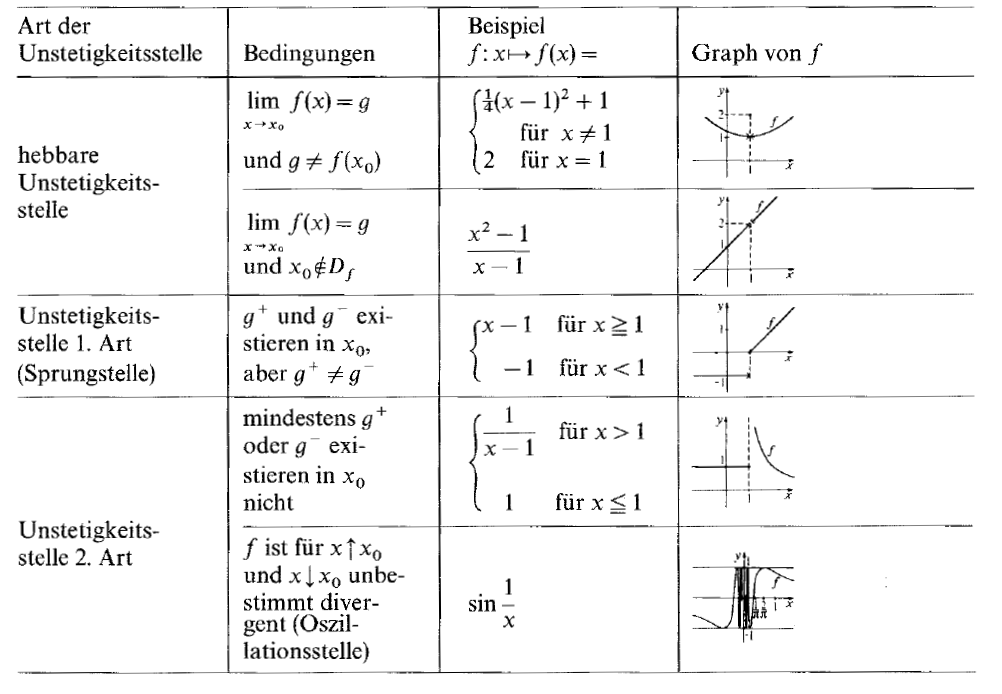
\includegraphics[width=0.9\linewidth]{Bilder/stetigkeit} \\

		\subsubsection{Übertragungsprinzip (Folgenprinzip)}
			$f$ besitzt an der Stelle $x_0$ Grenzwert $g$, wenn für jede gegen $x_0$\\
			konvergente Folge $< x_n >$ gilt: $\lim\limits_{x \to \infty} f(x_n) = g$ 
			
			\textbf{Beispiel} \\
				$f(x) = \frac{\vert x + 2 \vert}{2x+4}$ und $x_0 = -2$ \\
				\begin{tabular}{ll}
					linksseitig: & $x_n = x_0 - \frac{1}{n}$ für jedes x in f(x) einsetzen; \\
					& Grenzwert $g^-$ gegen $\infty$ bestimmen \\
					\\
					rechtsseitig: & $x_n = x_0 + \frac{1}{n}$ für jedes x in f(x) einsetzen; \\
					& Grenzwert $g^+$ gegen $\infty$ bestimmen \\
				\end{tabular}
			
		\subsubsection{Nullstellen bestimmen gemäss Bolzano (Bisektion)}
			$f(x)$ auf Intervall $[a;b]$ stetig, $f(a)$ und $f(b)$ haben versch. Vorzeichen \\
			$\rightarrow$ Es existiert (mindestens) eine 	Nullstelle $\xi$\\	
			NS mittels Bisektion (Intervallschachtelung) näherungsweise berechnen: \\
			
			\begin{tabular}{ll}
				(1) & $I_0 = [a ; b] = [a_0 ; b_0]$ gesamtes Intervall \\
				(2) & $I_0$ halbieren $\rightarrow m = \frac{a_0 + b_0}{2}$ \\
				(3) & Teil-Intervall mit Vorzeichenwechsel bestimmen: \\
				    & links: $f(a) \cdot f(m) < 0$ ; rechts: $f(b) \cdot f(m) > 0$ \\
				(4) & Teil-Intervall mit Vorzeichenwechsel: $I_1 = [a_1 ; b_1]$ \\
				(5) & Schritt (2) - (4) n mal wiederholen: $I_{n+1} \in I_n$ \\
				(6) & ... $\xi \in (a;b)$ mit $f(\xi) = 0$ (Nullstelle) \\
				(7) & $ \vert $Error$ \vert \leq \frac{b-a}{2^{n Schritte + 1}} $ \\
			\end{tabular}						
				
			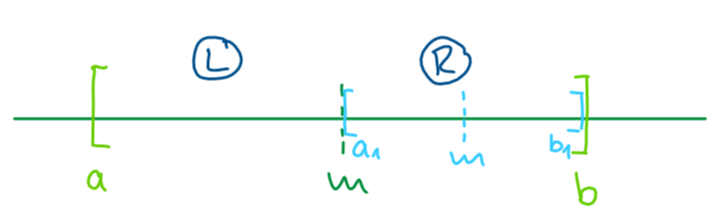
\includegraphics[width=0.9\linewidth]{Bilder/bisektion}
		
		\subsubsection{Spezielle Grenzwerte}	
			\begin{tabular}{lll}
				$\lim\limits_{x \to \infty} \frac{\sin(x)}{x} = 1$ &  $\lim\limits_{x \to \infty} (1 + \frac{a}{x})^x = \e^a$ & $\lim\limits_{x \to 0} \frac{\log_a(x+1)}{x} = \frac{1}{\ln(a)}$  \\
				\\
				$\lim\limits_{x \to 1} \frac{x}{1-\e^{-x}} = 1$ & $\lim\limits_{x \to \infty} \sqrt[x]{x} = 1$  & $\lim\limits_{x \to 0} (1+x)^{\frac{1}{x}} = 1$ \\
				\\
				$\lim\limits_{x \to \infty} \frac{(\ln(x))^\alpha}{x^\beta} = 0$ & $\lim\limits_{x \to 0^+} x \cdot \ln(x) = 0$  & $\lim\limits_{x \to 0} \frac{a^x -1}{x} = \ln(a)$ \\
				\\
				$\lim\limits_{x \to 0} \frac{\e^x - 1}{x} = 1$ & $\lim\limits_{x \to 0} \frac{(a+x)^\alpha -1}{x} = \alpha$  & $\lim\limits_{x \to 0+} z^z = 1$ \\
				\\
				$\lim\limits_{x \to 0+} x^{\sin(x)} = 1$ & $\lim\limits_{x \to 0+} y^{\beta} (\ln(y))^{\alpha} = 0 $ &  \\
			\end{tabular}
			\\
			\begin{tabular}{ll}
				$\lim\limits_{x \to \infty} \frac{x^\alpha}{a^{\beta x}} = 0 \; (a > 1; \alpha, \beta > 0)$  & $\lim\limits_{x \to \infty} \sum\limits _{k=0}^n q^k = 
					\begin{cases}			
						\infty & q \geq 1 \\
						\frac{1}{1-q} & \vert q \vert < 1
					\end{cases} $ \\ 
			\end{tabular}

		\subsubsection{Asymptotenbestimmung}
			Asymptote einer gebrochen rationalen Funktion $f(x) = \frac{a_nx^n + ... + a_1x + a_0}{b_mx^m + ... + b_1x + b_0}$\\
			bestimmen gemäss:
			
			\begin{tabular}{|l|l|l|l|}
				\hline
				& $m > n$ & $m = n$ & $m < n$ \\
				\hline
				$\lim\limits_{x\to \pm \infty} r(x)$  & 0 & $\frac{a_n}{b_m}$ & $\infty$ oder $-\infty$ \\
				\hline
				Asymptote & x-Achse & $\parallel x, g(x) = \frac{a_m}{b_n}$ & ganzrat. Teil \\
				          &         &                                        & der Polynomdiv. \\
				\hline
				Konv./Div. & Konvergenz & Konvergenz & Divergenz \\
				\hline
			\end{tabular}
			
		\subsubsection{Grenzwerte von rekursiven Folgen}
			Anwendung des Bolzano-Prinzips!  Beispiel: $a_1 = \frac{1}{4}$ ; $a_{n+1} = a_n^2 + \frac{1}{4}$ \\
			
			\begin{tabular}{ll}
				1. & Monotonie \\
				   & beweisen mit Ansatz $a_{n+1} \geq a_n$ bzw. $a_{n+1} \leq a_n$ \\
				\\
				2. & Beschränktheit \\
				   & erste Schranke = erster Wert der Reihe \\
				   & Zweite Schranke: Annahme, es gibt Grenzwert g und er ist \\
				   & sup / inf \\
				\\
				   & Grenzwertgleichung: $a_{n+1} = a_n ^2 + \frac{1}{4}$  $(n \rightarrow \infty)$ $\Rightarrow g = g^2 + \frac{1}{4}$ \\
				   & Gleichung nach g auflösen \\
				   & $\Rightarrow$ Wenn es ein sup / inf gibt, dann ist es das berechnete g $\in \mathbb{R}$\\
				\\
				3. & Beweisen (oder widerlegen), dass g sup / inf ist \\
				   & Ansatz: $a_n \leq g$ bzw. $a_n \geq g$ mit vollst. Induktion beweisen \\
			\end{tabular}

	\vfill\null
	\pagebreak
